\subsection{Bahnplanung}
Zunächst einige relevante Definitionen:
\begin{itemize}
\item \red{Konfiguration $K$}: vollständige, eindeutige Beschreibung
des Zustands eines Roboters $A$, z.B.
\begin{itemize}
\item im euklidischen Raum durch seine Position und Orientierung
\item im Gelenkwinkelzustandsraum durch die Werte der Gelenke
\end{itemize}
\item \red{Konfigurationsraum $\mathbb{K}$}: Raum aller
möglichen Konfigurationen des Roboters $A$
\item \red{Weg} des Roboter $A$ von der Konfiguration $K_{Start}$ zu $K_{Ziel}$ ist eine stetige Abbildung:
\begin{align*}
\tau: [0, 1] \rightarrow \mathbb{K}\\
\tau(0) = K_{Start} ,\tau(1) = K_{Ziel}
\end{align*}
\item \red{Einschränkung} für den Roboter $A$ ist eine Abbildung:
\begin{align*}
\lambda : \mathbb{K} \rightarrow [0, 1]
\end{align*} 
\item \red{Arbeitsraumhindernis $H$}: Raum, welcher von
einem Objekt im Arbeitsraum eingenommen wird
\item \red{Konfigurationsraumhindernis $\mathbb{K}_{H_i}$}: Menge aller
Punkte des Konfigurationraumes, welche innerhalb eines
Arbeitsraumhindernisses $H_i$ liegen:
\begin{align*}
\mathbb{K}_{H_i} = {K \in \mathbb{K} | K \in H_i}
\end{align*}
\item \red{Hindernisraum $\mathbb{K}_{H_i}$}: Menge aller
Konfigurationsraumhindernisse:
\begin{align*}
\mathbb{K}_H =\bigcup_i \mathbb{K}_{H_i}
\end{align*}
\item \red{Freiraum $\mathbb{K}_F$}: Menge aller Punkte aus $\mathbb{K}$, welche nicht im
Hindernisraum liegen:
\begin{align*}
\mathbb{K}_F = \mathbb{K}\backslash \mathbb{K}_H
\end{align*}
\item \red{kollisionsfreier Weg $\tau$}: Weg mit $Bild(\tau) \subseteq \mathbb{K}_F$, also ein Pfad welcher alle Einschränkungen erfüllt
\end{itemize}
Bei einer Bahnplanung im Konfigurationsraum werden Bewegungen eines Roboters als \red{Trajektorie im Konfigurationsraum}, d.h. als Zustandsänderungen über die Zeit
relativ zu einem stationären Koordinatensystem (kartesischer Raum, Gelenkwinkelraum) aufgefasst:
\begin{itemize}
\item Gegeben: $K_{Start}$ = Startkonfiguration, $\land_{Ziel}$ = Menge der Zieleinschränkungen
\item Gesucht: Kollisionsfreier Weg $\tau$ von $K_{Start}$ nach $K$ mit $\lambda(K)=1 \forall \lambda \in \land_{Ziel}$
\item Bedingungen: i.A. Gütekriterien, Neben-,Rand- sowie Zwangsbedingungen
\end{itemize}
Hierbei sei angemerkt, dass von Roboter und Umwelt zu einem Punkt im Konfigurationsraum abstrahiert wird. Die Kollisions- bzw. Einschränkungsüberprüfung stellt eine Blackbox
\begin{align*}
f: \mathbb{K} \rightarrow \{0, 1\}\\
\text{Beispiel:} f(K) = \bigwedge\limits_{\varv \in \land_{Weg}}^{} \varv(K) \geq \varepsilon(\varv)
\end{align*}
dar. Bei Entwicklung allgemeiner Planungsverfahren auf Basis dieser Abstraktion entspricht die Bahnplanung einer Suche nach einer stetigen Verbindung zweier Punkte im
Konfigurationsraum. Eine explizite Beschreibung des Freiraums ist nicht notwendig, d.h. das Suchverfahren ist unabhängig von der Struktur und Repräsentation des Freiraums.

\subsubsection*{Simpler Rapidly-exploring Random Tree (RRT) Planer}
\paragraph*{RRT-Algorithmus}
Wie bereits zu Anfang des Kapitels erwähnt, bringt die humanoide Servicerobotik zahlreiche Anforderungen mit sich, sowie die Manipulation beliebiger Objekte, das selbstständige Lösen komplexer Aufgaben und den Einsatz im menschlichen Umfeld, d.h. humanoide Serviceroboter müssen in einer sehr komplexen Umgebung agieren und verfügen über sehr viele Freiheitsgrade (der Roboter Albert II beispielsweise hat 13df,  6 im Arm, 3 in der Plattform und 4 in der Hand. Daraus ergibt sich ein 13-dimensionaler Konfigurationsraum $\mathbb{R}^{13}$ als reellwertige Grundlage).
Ein Bahnplanungsalgorithmus, der hiermit umgehen kann ist der RRT = Rapidly-exploring Random Tree\footnote{[LaValle/Kuffner99]: Randomized Kinodynamic
Planning}, welcher zur effizienten Durchsuchung hoch-dimensionaler Räume entwickelt wurde. Er ist geeignet für holonome und nicht-holonome Problemstellungen mit Einschränkungen. Es wird inkrementell eine Baumstruktur aufgebaut und dabei der erwartete Abstand eines Punkts zu einem Knoten im Baum minimiert. Wenn die Zeit $t$ gegen unendlich geht kommt man beliebig nah an jeden beliebigen Punkt. Der Algorithmus erreicht eine hohe Geschwindigkeit durch schnelles Wachstum in nicht explorierte Bereiche. Die Wurzel ist ein Punkt im 13-dimensionalen Konfigurationsraum. Pseudocode ist in Algorithmus \ref{alg:rrt}. 
Eine graphische Veranschaulichung zeigt \autoref{fig:rrt}.
Der Knoten mit der größten Voronoi-Region hat jeweils die größte Wahrscheinlichkeit, als nächstes erweitert zu werden (\textbf{Voronoi-Bias}). Da am Anfang die Voronoi-Gebiete am
Randbereich groß sind findet zunächst eine rasche Exploration und dann eine Verfeinerung statt (vgl. Abbildungen \ref{fig:vb} und \ref{fig:vb1}).
\begin{algorithm}
  \caption{RRT
    \label{alg:rrt}}
  \begin{algorithmic}[1]
    %\Require{$x$ and $y$ are packed \DNA strings of equal length $n$}
    %\Statex
    \Statex {BUILD\_RRT}($K_{Start}, n, \varepsilon$)
      \State $T$.init($K_{Start}$) \Comment{Neuer Baum mit Startkonfiguration in der Wurzel}
      \For{$k = 1 \textrm{ to } n$}
        \Let{$K_{Zuf}$}{RAND\_CONF()} \Comment{Gleichverteilt zufällige Erzeugung einer Konfiguration}
        \Let{$K_{Nahe}$}{NEAREST\_VERTEX($K_{Zuf}, T$)} \Comment{Bestimmung des nächsten Knotens}
        \Let{$K_{Neu}$}{EXTEND($K_{Nahe}, K_{Zuf}, \varepsilon$)} \Comment{Erzeugung einer neuen Konfiguration}
        \State $T$.add\_vertex($K_{Neu}$)
        \State $T$.add\_edge($K_{Nahe}, K_{Neu}$)
      \EndFor
      \State \Return{$T$}
    %\EndFunction
  \end{algorithmic}
\end{algorithm}

%Beispiel für Verwendung des Algorithmus-Packages
%\begin{algorithm}
%  \caption{Counting mismatches between two packed \DNA strings
%    \label{alg:packed-dna-hamming}}
%  \begin{algorithmic}[1]
%    \Require{$x$ and $y$ are packed \DNA strings of equal length $n$}
%    \Statex
%    \Function{Distance}{$x, y$}
%      \Let{$z$}{$x \oplus y$} \Comment{$\oplus$: bitwise exclusive-or}
%      \Let{$\delta$}{$0$}
%      \For{$i \gets 1 \textrm{ to } n$}
%        \If{$z_i \neq 0$}
%          \Let{$\delta$}{$\delta + 1$}
%        \EndIf
%      \EndFor
%      \State \Return{$\delta$}
%    \EndFunction
%  \end{algorithmic}
%\end{algorithm}
\begin{figure}[h!]
	\centering
	\begin{subfigure}{.4\textwidth}
		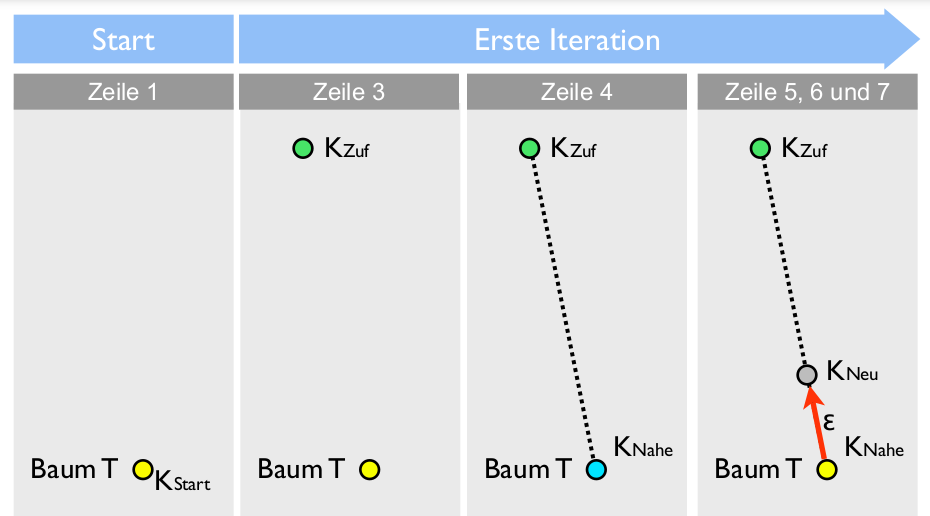
\includegraphics[width=\textwidth]{figures/ch04_rrt1.png}
	\end{subfigure}
	\begin{subfigure}{.4\textwidth}
		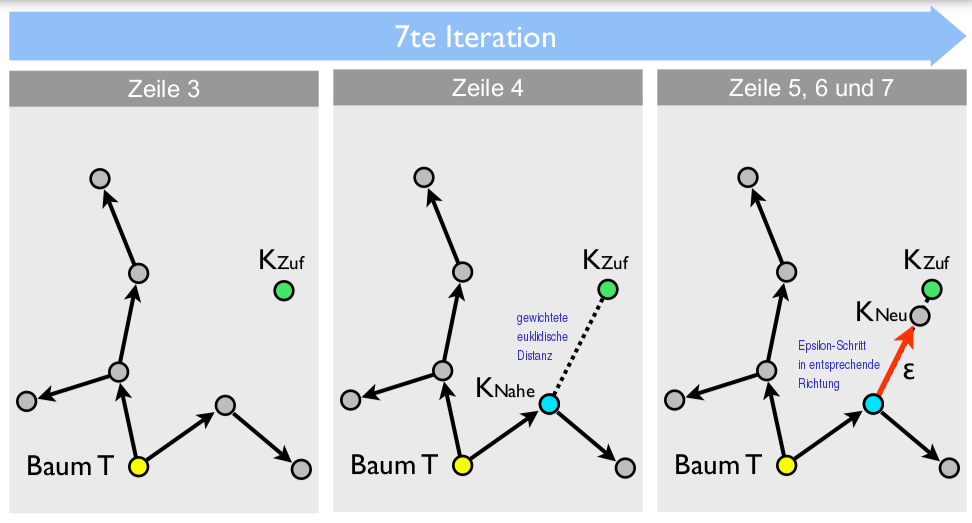
\includegraphics[width=\textwidth]{figures/ch04_rrt2.png}
	\end{subfigure}
	\caption{Graphische Veranschaulichung - RRT}
	\label{fig:rrt}
\end{figure}
\begin{figure}[h!]
	\centering
	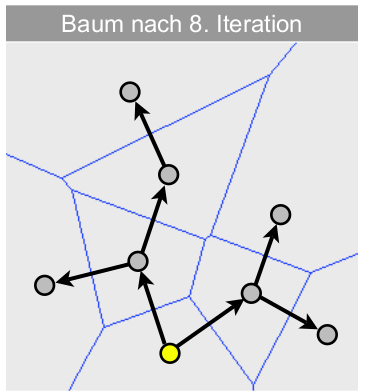
\includegraphics[width=.15\textwidth]{figures/ch04_voronoi.png}
	\caption{Voronoi-Bias -- Detail}
	\label{fig:vb}
\end{figure}
\begin{figure}[h!]
	\centering
	\begin{subfigure}{.3\textwidth}
		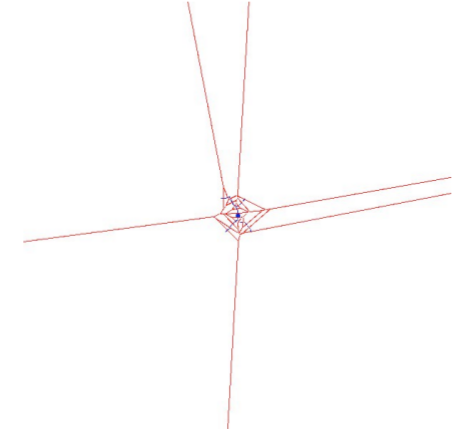
\includegraphics[width=\textwidth]{figures/ch04_voron1.png}
	\end{subfigure}
	\begin{subfigure}{.3\textwidth}
		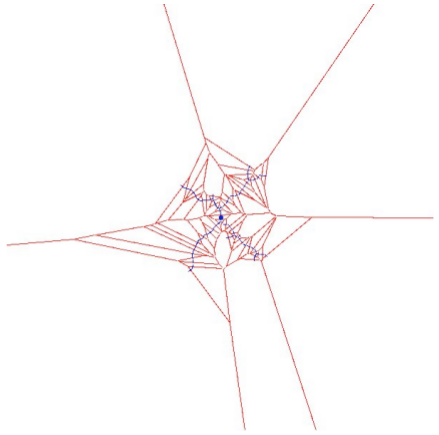
\includegraphics[width=\textwidth]{figures/ch04_voron2.png}
	\end{subfigure}
	\begin{subfigure}{.3\textwidth}
		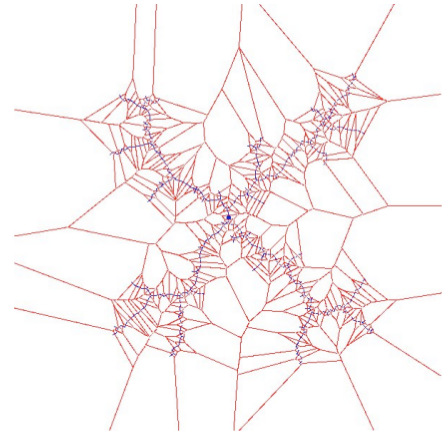
\includegraphics[width=\textwidth]{figures/ch04_voron3.png}
	\end{subfigure}
	\begin{subfigure}{.3\textwidth}
		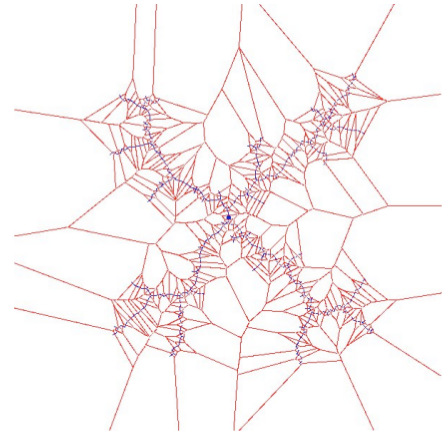
\includegraphics[width=\textwidth]{figures/ch04_voron3.png}
	\end{subfigure}
	\begin{subfigure}{.3\textwidth}
		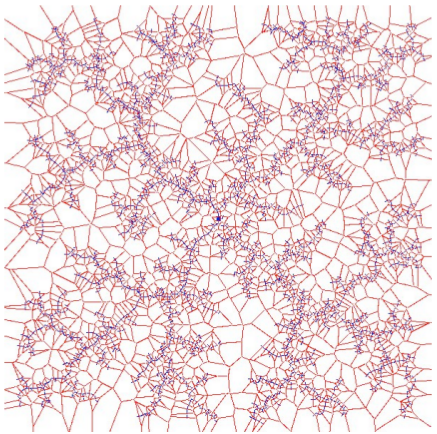
\includegraphics[width=\textwidth]{figures/ch04_voron5.png}
	\end{subfigure}
	\begin{subfigure}{.3\textwidth}
		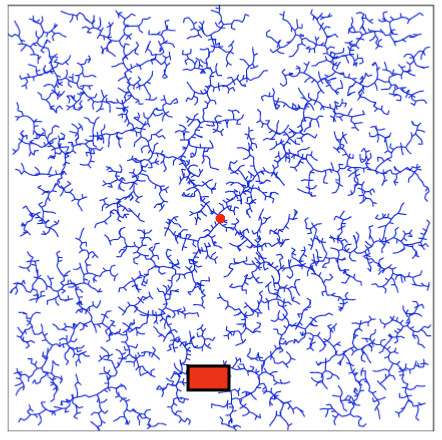
\includegraphics[width=\textwidth]{figures/ch04_voron6.png}
	\end{subfigure}
	\caption{Voronoi-Bias}
	\label{fig:vb1}
\end{figure}
RRT: Zusammenfassung
\begin{itemize}
\item Allgemeines Verfahren zur Durchsuchung hoch-dim. Räume
\item Online-Verfahren
\item Approximation des Suchraums durch eindimensionale Struktur: Baum
\item Rasche Exploration des Suchraums: Voronoi-Bias
\item Probabilistische (oder deterministische) Stichprobenerzeugung
\item Einfach zu implementieren, nur wenige Parameter ($\varepsilon$, Distanzfunktion auf $\mathbb{K}$)
\end{itemize}
\newpage
\paragraph{Anwendung in der Bahnplanung} Es sind drei Fragen zu klären:
\begin{enumerate}
\item Wie Einschränkungen berücksichtigen?
\item Wie zielgerichtet suchen?
\item Wie kollisionsfreie Wege erzeugen?
\end{enumerate}
Hierzu muss der Basisalgorithmus erweitert werden:
\begin{itemize}
\item Es werden nur Konfigurationen hinzugefügt, die alle Einschränkungen erfüllen.
\item Bei der Stichprobenerzeugung werden mit einer bestimmten Wahrscheinlichkeit Zielkonfigurationen generiert, der Baum wächst in die Richtung der Zielkonfigurationen.
\item Der Planungsprozess ist beendet, wenn die letzte Konfiguration die Zieleinschränkungen erfüllt.
\end{itemize} 
\textbf{Frage 1 \& 2: Einbeziehung von Einschränkungen und Umgang mit Kollisionen} (vgl. \autoref{fig:einschr})
\begin{itemize}
\item $K_{Neu}$ wird übernommen, wenn alle Einschränkungen zwischen $K_{Nahe}$ nach $K_{Neu}$ erfüllt sind
\item Keine Distanz, nur Ja / Nein
\item Kollisionen auf Grundlage eines Geometriemodells der Objekte (Standard: 3D-Dreiecksnetze)
\item Kollisionsüberprüfung: mindestens zwei Dreiecke schneiden sich (oder 1. Objekt in 2. komplett enthalten)
\item hierzu gibt es optimierte Algorithmen, ist vergleichsweise langsam
\end{itemize}
\begin{figure}[h!]
	\centering
	\begin{subfigure}{.3\textwidth}
		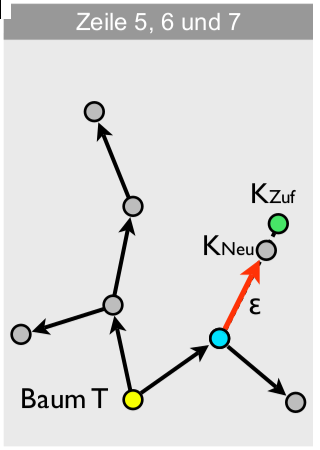
\includegraphics[width=\textwidth]{figures/ch04_Kol.png}
		\caption{$K_{Zuf}$ könnte auch schon ZK erfüllen, überprüfe dies, falls ja ist Planung beendet}
		\label{kol}
	\end{subfigure}
	\begin{subfigure}{.5\textwidth}
		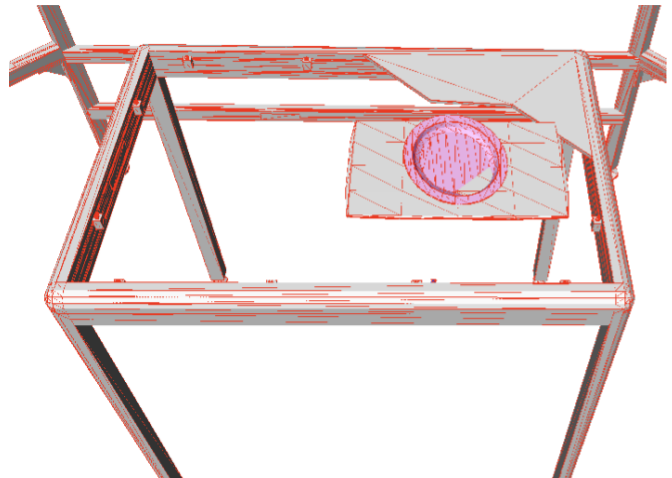
\includegraphics[width=\textwidth]{figures/ch04_Kol1.png}
		\caption{Der Roboter \glqq weiß\grqq{} um das Vorhandensein des Tisches nur über Einschränkungen; es wird der Schnitt zweier Dreiecke berechnet; da hier der Teller im Tisch hängt wird diese Konfiguration dem Baum nicht hinzugefügt}
	\end{subfigure}
	\caption{Einbeziehung von Einschränkungen und Kollisionen}
	\label{fig:einschr}
\end{figure}
\textbf{Frage 3: Wie zielgerichtet planen?}
Wie in \autoref{vb1} dargestellt definiert die Menge der Zieleinschränkungen i.d.R. ein stark begrenztes Gebiet in $\mathbb{K}$ (roter Bereich im 6. Panel der Abbildung), z.B. endliche Menge von gültigen Zielkonfigurationen. Somit ist die Wahrscheinlichkeit eine Zielkonfiguration zufällig zu erzeugen minimal, es dauert recht lange bis der Baum in den betreffenden Bereich reinwächst.
Daher ist die in Algorithmus \autoref{alg:rrt-detail} dargestellte Modifikation der Stichprobenerzeugung sinnvoll (vgl. \autoref{rrt-erw}). Der resultierende Algorithmus ist Algorithmus \ref{alg:rrt-erw}.\\
\begin{algorithm}
  \caption{Detail
    \label{alg:rrt-detail}}
  \begin{algorithmic}[1]
    %\Require{$x$ and $y$ are packed \DNA strings of equal length $n$}
    %\Statex
    \Statex {RAND\_CONF}($f_{Ziel}, \delta$) \Comment{z.B. $\delta = 0.01$}
      \State $P \thicksim U(\left[0,1\right])$
      \If{$P < \delta$}
      	\State \Return{$K \in \mathbb{K}: f_{Ziel}(K) = 1$}
      \Else
      	\State \Return{$K \thicksim U(\mathbb{K})$}
      \EndIf
    %\EndFunction
  \end{algorithmic}
\end{algorithm}
\begin{figure}[h!]
	\centering
	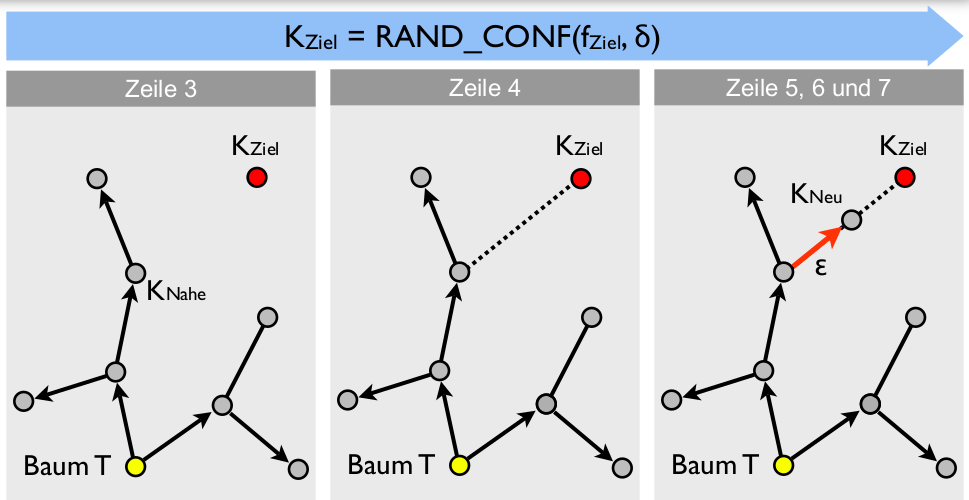
\includegraphics[width=.5\textwidth]{figures/ch04_rrt-erw.png}
	\caption{Erweiterung -- Zielgerichtet planen mit RRT}
	\label{rrt-erw}
\end{figure}
\begin{algorithm}[h!]
  \caption{Simpler RRT Planer
    \label{alg:rrt-erw}}
  \begin{algorithmic}[1]
    \Statex {RRT\_SIMPLE}($K_{Start}, \textcolor{red}{f_{Ziel}}, \textcolor{red}{f_{Weg}}, \varepsilon, \textcolor{red}{\delta}$)
      \State $T$.init($K_{Start}$) \Comment{$f_{Ziel}$ ist Blackbox für Zieleinschränkungen}
      \For{$k = 1 \textrm{ to } MAX$}
        \Let{$\textcolor{red}{K_{Zuf}}$}{\textcolor{red}{RAND\_CONF($f_{Ziel}, \delta$)}} 
        \Let{$K_{Nahe}$}{NEAREST\_VERTEX($K_{Zuf}, T$)} \Comment{$f_{Weg}$ ist Blackbox für Einschränkungen}
        \Let{$K_{Neu}$}{EXTEND($K_{Nahe}, K_{Zuf}, \varepsilon$)} \Comment{Erzeugung einer neuen Konfiguration}
        \If{\textcolor{red}{$f_{Weg}(K_{Neu}) = 1$}}
        	\State $T$.add\_vertex($K_{Neu}$)
        	\State $T$.add\_edge($K_{Nahe}, K_{Neu}$)
        	\If{\textcolor{red}{$f_{Ziel}(K_{Neu}) = 1$}} \Comment{Lösungspfad: Rückverfolgung der Elternknoten beginnend mit dem letzten Knoten}
        		\State \Return{$T$, Gefunden}
        	\EndIf
        \EndIf
      \EndFor
      \State \Return{$T$, Nicht gefunden}
  \end{algorithmic}
\end{algorithm}
\newpage \noindent
\textbf{Beispiel für die Anwendung des Simplen RRT Planers}: Holonome Planung für einen Roboterarm mit 7 Freiheitsgraden (vgl. \autoref{fig:rrt-bsp})
\begin{itemize}
\item Konfigurationsraum $\mathbb{K}= \left[0,1\right]$ (Gelenkwinkelbereich $\left[-170°, +170°\right]$ wird auf Bereich $\left[0,1\right]$ normiert)
\item Distanzfunktion auf $\mathbb{K}$: $d(k,s) = \sum\limits_{i = 1...7} w_i (k_i - s_i)$
\item Gewichtsvektor $w=(1.5,1.5,1.5,1.25,1,1,1)$
\item $\varepsilon = 0.001, \delta = 0.01$ (Schrittweite: mit welcher WK man Zielkonfiguration erzeugt)
\item $f_{Ziel}(K) = 1 \Leftrightarrow K = K_ {Ziel}$
\item $f_{Weg}(K) = 1 \Leftrightarrow K$ ist kollisionsfrei
\end{itemize}
\begin{figure}[h!]
	\centering
	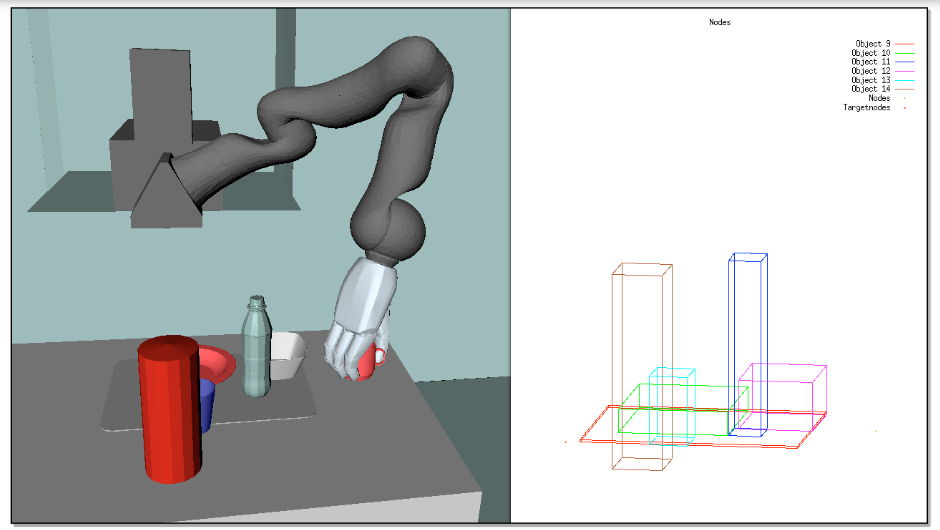
\includegraphics[width=.5\textwidth]{figures/ch04_rrt-bsp.png}
	\caption{Beispiel für die Anwendung des Simplen RRT Planers: Arm bewegt sich relativ weich, auf recht glatter Bahn}
	\label{fig:rrt-bsp}
\end{figure}
\subsubsection*{Pfadglättung und Hinderniserweiterung}
\textbf{Reale Anwendung}: Der Planer kann so nicht direkt eingesetzt werden
\begin{itemize}
\item Glättung notwendig, da Weg nicht glatt
\item Hinderniserweiterung notwendig, da kleine Abweichungen von der Bahn zu Kollisionen führen können
\end{itemize}
\textbf{Verringerung der Länge des Lösungswegs} (siehe \autoref{fig:abkuerz}):
\begin{itemize}
\item Zufällige Wahl zweier Knoten im Lösungsweg
\item Überprüfung der Verbindung beider Knoten auf Einhaltung der Einschränkungen
\item Falls die Verbindung geringere Kosten aufweist als der entsprechende Teillösungspfad, Verbindung der beiden Knoten und Löschen der dazwischenliegenden Knoten aus dem Lösungspfad
\end{itemize}
\begin{figure}[h!]
	\centering
	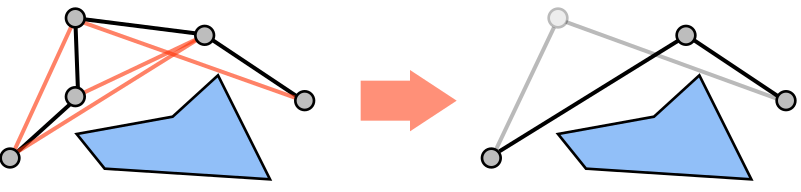
\includegraphics[width=.5\textwidth]{figures/ch04_abkuerz.png}
	\caption{rot -- g\"{u}ltige Abk\"{u}rzungen  $\rightarrow$ Kollisionsfreiheit muss erhalten bleiben; normaler Lösungspfad hat etwa 1000 Knoten}
	\label{fig:abkuerz}
\end{figure}
\textbf{Hinderniserweiterung} zur Berücksichtigung eines Toleranzbereichs im Planungsprozess durch Vergrößerung der Hindernisse
\begin{itemize}
\item Gründe:
\begin{itemize}
\item Diskretisierung des Konfigurationsraums bzw. Abtastung von Trajektorien
\item Fehler der Objektlokalisierung: Kalibrierung des Roboters, Objekterkennung/-verfolgung
\item Abweichungen in der Bewegung: Rutschen, lockere Seilzüge, Modellierung, Impedanzregelung, Interpolationsart
\item Padding: Rand um beliebiges Hindernis festlegen (oft vorhandener Parameter in State-of-the-Art Bahnplanungs-Bibliotheken), vor allem für dünne Gegenstände sinnvoll
\end{itemize}
\item Probleme:
\begin{itemize}
\item Künstliche Einschränkung des Arbeitsraums
\item $\varepsilon$ muss klein gewählt werden
\ita Annahme: Wenn der Roboter an einem Punkt hindernisfrei ist und 0.5mm weiter auch, dann auch dazwischen
\ita Kann zu Problemen führen; kontinuierliche Kollisionserkennung als Workaround, Distanzberechnung erlaubt exakte Bestimmung aber super aufwendig
\item Erzeugung von Narrow-Passages: Lücken dicht gemacht durch Hindernisvergrößerung, eventuell keine gültige Lösung mehr vorhanden
\end{itemize}
\end{itemize}
\textbf{Zusammenfassung -- Simpler RRT Planer}:
\begin{itemize}
\item Probabilistisch vollständig
\item Uniforme Stichprobenverteilung → Bereiche im Suchraum mit geringem Lebesgue-Maß, z.B. Narrow Passages, werden nicht abgedeckt
\item Hohe Laufzeitvarianz
\item Kein problemspezifisches Wissen
\item Ineffiziente Ergebnispfade → Glättung notwendig
\item[$\Rightarrow$] \textcolor{red}{Manipulation:} Einschränkungen können Unterräume mit Lebesgue-Maß 0 erzeugen
\begin{itemize}
\ita Modifikation notwendig
\ita Blackbox-Formulierung der Einschränkungen problematisch
\end{itemize}
\end{itemize}
\subsubsection*{TC-RRT: Planung mit Task Constraints}
Zweck: Berücksichtigung von Einschränkungen im Planungsprozess\\
Wiederholung:
\begin{itemize}
\item Ziele haben gleiche Struktur wie Einschränkungen
\item Kollisionsfreiheit ist eine Einschränkung
\item Erweiterung des Blackbox-Konzepts auf Einschränkungen möglich.\\
Problem: Narrow-Passages und Nullmengen treten sehr viel häufiger als bei Kollisionen auf.
\ita spezielle Methoden zur Berücksichtigung von Einschränkungen nötig
\end{itemize}
\textbf{Ansatz}\footnote{basiert auf [Stilman07], [Berenson09]}:
\begin{itemize}
\item Wesentliches Konzept: Erweiterung der Einschränkung-Definition um Richtungsfunktion im Taskraum (\glqq Öffnen der Blackbox\grqq)
\item Richtungsfunktion berechnet den Abstand und den Richtungsvektor zu einem Zustand, der die Einschränkung erfüllt
\item Verwendung lokaler Optimierung mit Gradientenabstieg um von beliebiger Konfiguration zu einer gültigen Konfiguration zu kommen
\item Funktioniert sehr gut in der Praxis (oftmals einfache, konvexe Einschränkungen)
\item Constraint-Definition durch Angabe der Richtungsfunktion: $\lambda : \mathbb{K} \rightarrow \mathbb{K}_{Kart} \times \mathbb{R}$
\begin{itemize}
\item $\mathbb{K}_{Kart}$ ist der kartesische Arbeitsraum (z.B. $\mathbb{R}^3, \mathbb{R}^6$)
\item Hier: $\lambda(K) = \begin{pmatrix}x &y& z& rx& ry& rz& a)\end{pmatrix}$ mit $rx, ry, rz$ skalierte Rotationsachsen
\end{itemize}
\item Ersetzung der Extend-Funktion durch ConstrainedExtend
\item ConstrainedExtend berechnet neue Konfiguration, die alle Einschränkungen erfüllt
\item 3 Methoden zur Berechnung der ConstrainedExtend-Funktion:
\begin{itemize}
\item Randomized Gradient Descent (RGD)
\item First Order Retraction (FR)
\item Tangent Space Sampling (TS)
\end{itemize}
\end{itemize}
\textbf{Randomized Gradient Descent (RGD)} (vgl. \autoref{rgd}):
\begin{itemize}
\item Toleranzwert für Einschränkungen: $\alpha$
\item Zufällige Bestimmung von $n$ Nachbarn von $K_S$ (in Hyperkugel mit Radius $d_{max}$ )
\item Falls minimale Distanz der Nachbarn kleiner als die Distanz von $K_S$, ersetze $K_S$ mit dem Nachbarn mit kleinster Distanz
\item Wiederholen bis maximale Iterationszahl erreicht oder die Distanz von $K_S < \alpha$ ist
\item[$\Rightarrow$] Keine Richtungsinformation notwendig (einzige gültige Stichproben liegen in Ebene)
\end{itemize}
\textbf{First Order Retraction (FR)} (vgl. \autoref{fr}):
\begin{itemize}
\item Toleranzwert für Einschränkungen: $\alpha$
\item Speichern von $K_S$ in $K_O$
\item Berechnen der Distanz $\Delta x$ von $K_S$
\item \glqq Einfahren\grqq{} von $K_S$: $K_S = K_S - J(K_S)^\dagger \Delta x$ (Bemerkung: die Notation $A^\dagger$ bezeichnet die Matrix, die durch Transponierung und Konjugation einer gegebenen komplexen Matrix $A$ entsteht)
\item Iterieren bis die Distanz $< \alpha$ oder Abstand $|K_O - K_S |$ größer als $|K_O - K_{Nahe}|$
\end{itemize}
\begin{figure}[h!]
	\centering
	\begin{subfigure}{.25\textwidth}
		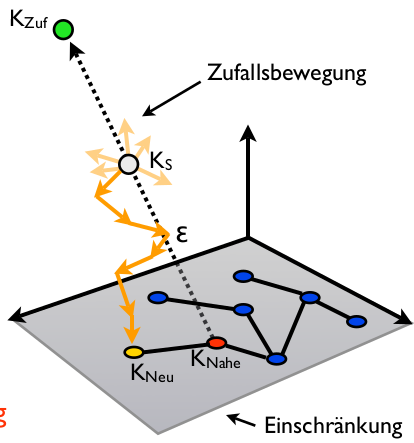
\includegraphics[width=\textwidth]{figures/ch04_rgd.png}
		\caption{Randomized Gradient Descent}
		\label{rgd}
	\end{subfigure}
	\begin{subfigure}{.25\textwidth}
		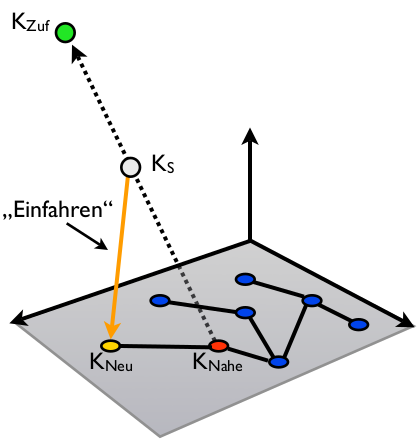
\includegraphics[width=\textwidth]{figures/ch04_fr.png}
		\caption{First Order Retraction}
		\label{fr}
	\end{subfigure}
	\caption{Methoden zur Berechnung der ConstrainedExtend-Funktion}
	\label{fig:rrt}
\end{figure}
\autoref{fig:sp-erz} stellt verschiedene Methoden der Stichprobenerzeugung gegenüber.
\begin{figure}[h!]
	\centering
	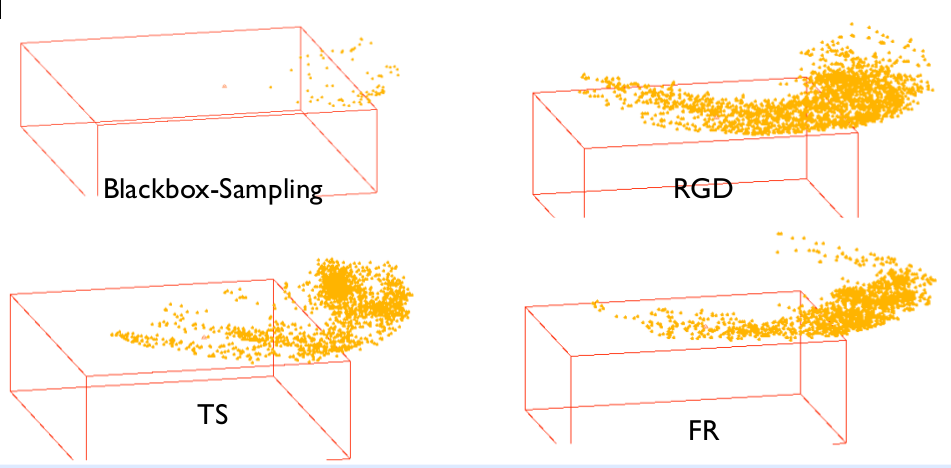
\includegraphics[width=.5\textwidth]{figures/ch04_sp-erz.png}
	\caption{Vergleich der Stichprobenerzeugung: Jacobimatrix-basierte Ansätze bei komplexeren Einschränkungen im Vorteil}
	\label{fig:sp-erz}
\end{figure}\\
Der RGD wird beispielsweise in IPoR II verwendet, wie in \autoref{fig:rgd-ipor} dargestellt.
\begin{figure}[h!]
	\centering
	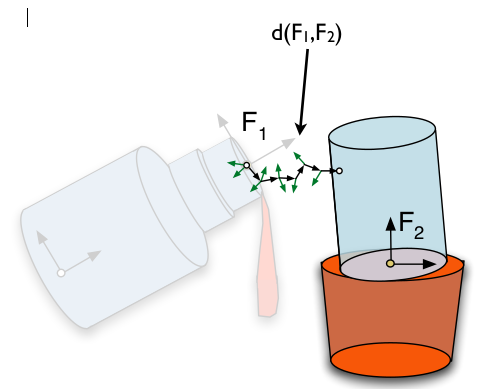
\includegraphics[width=.3\textwidth]{figures/ch04_rgd-ipor.png}
	\caption{RGD mit Distanz $d(F_1 ,F_2)$}
	\label{fig:rgd-ipor}
\end{figure}
\newpage
\textbf{RRT -- Erweiterungen}:
\begin{itemize}
\item Connect-Heuristik:
\begin{itemize}
\item Multiple Extend-Schritte in einer Iteration
\end{itemize}
\item Bidirektional:
\begin{itemize}
\item Wachsen eines RRTs in der Start- und Zielkonfiguration
\item Bäume wachsen aufeinander zu
\item Planungsproblem gelöst, wenn Bäume verbunden
\item Balanciert: gleiche Anzahl Knoten in beiden Bäumen
\end{itemize}
\item dd-RRT [Jaillet05]:
\begin{itemize}
\item Verwendung einer nicht-uniformen Stichprobenverteilung auf der Basis des aktuellen Suchbaums $\rightarrow$ Besseres Verhalten in eingeschränkten Regionen
\end{itemize}
\end{itemize}
\subsection{Griffklassifikation}
Bei IPoR II findet eine simple Abbildung auf Greifaktionen statt:
\begin{itemize}
\item Klassifikation des menschlichen Griffs im Segmentierungspunkt
\item Abbildung auf vordefinierten Griff der gleichen Klasse für Roboterhand
\item Bestimmung eines optimalen Griffs in Simulation
\item Ausführung auf Roboter
\end{itemize}
Für die Klassifikation des menschlichen Griffs gibt es z.B. folgende Ansätze:
\begin{itemize}
\item Klassenhierarchie nach Cutkosky
\item Training einer Support Vector Machine in jeder Hierarchieebene (10)
\item Hierarchische Auswertung der Support Vector Machines
\end{itemize}
\subsubsection*{Cutkosky-Hierarchie}
Die Cutkosky-Hierarchie ist in Abbildung \ref{fig:ch04_cuthie} dargestellt.
\begin{figure}[ht]\centering 
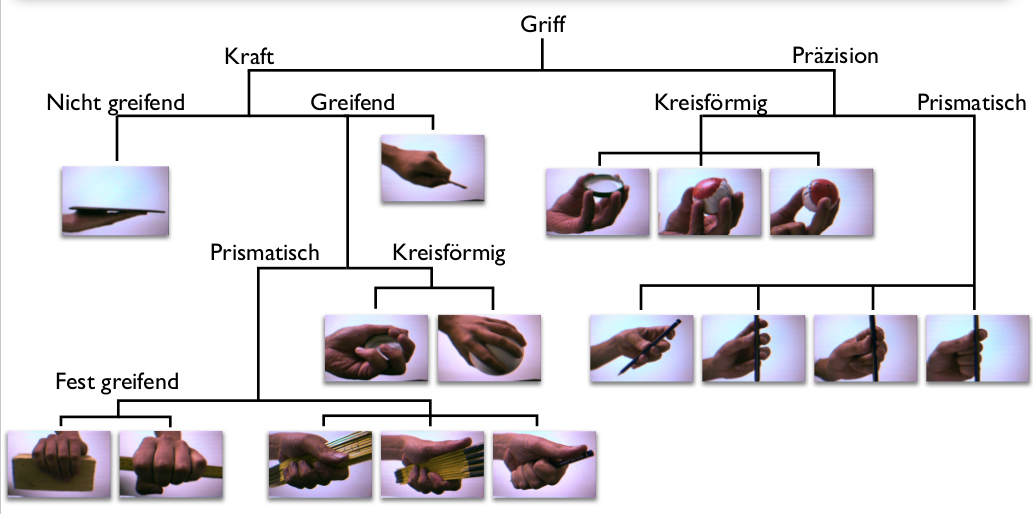
\includegraphics[width=0.6\linewidth]{figures/ch04_cutkosky.png}
\caption{Die Cutkosky-Hierarchie}
\label{fig:ch04_cuthie}
\end{figure}
Die in Abbildung \ref{fig:ch04_netztopo} gezeigte hierarchische Netztopologie reflektiert Griffklassifikation nach Cutkosky. Jedes Netz wird mit entsprechenden Beispielen trainiert.
\begin{figure}[ht]\centering 
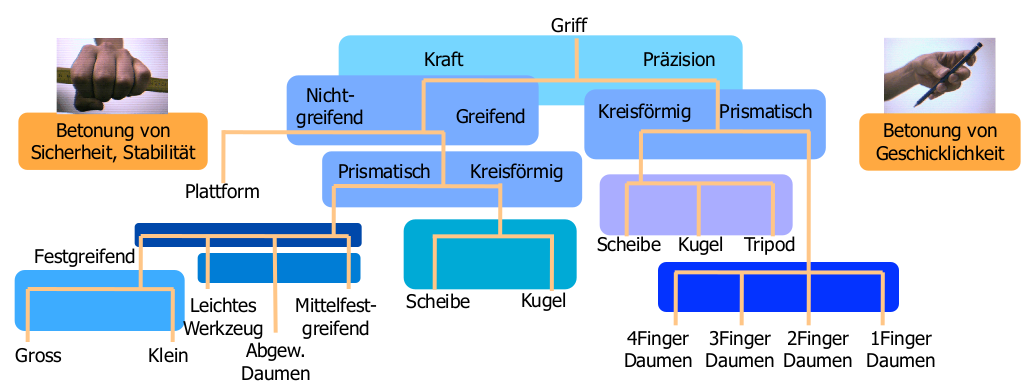
\includegraphics[width=0.6\linewidth]{figures/ch04_netztopo.png}
\caption{Hierarchische Netztopologie}
\label{fig:ch04_netztopo}
\end{figure}
\subsection{Griffplanung}
Zunächst einige relevante Definitionen:
\begin{itemize}
\item \red{Ziel}: Berechnung eines Griffs, d.h. Menge von Kontaktstellen zwischen Roboter und Objekt
\item \red{Kontaktstellen}($\rightarrow$ Geometrisches Objektmodell, vgl. Abbildung \ref{fig:ch04_griff}):
\begin{figure}[ht]\centering 
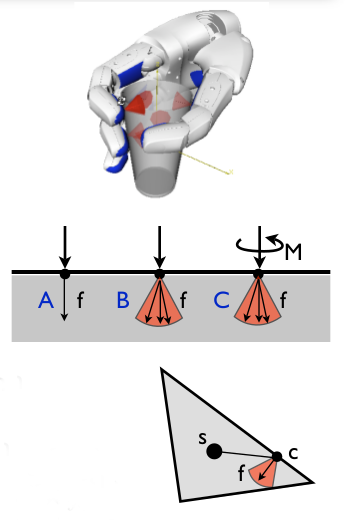
\includegraphics[width=0.3\linewidth]{figures/ch04_griff.png}
\caption{Griffplanung}
\label{fig:ch04_griff}
\end{figure}
\begin{itemize}
\item Punktkontakt ohne Reibung (\textcolor{blue}{A})
\item Starrer Punktkontakt mit Reibung (\textcolor{blue}{B})
\item Nicht-starrer Punktkontakt mit Reibung (\Gu soft finger contact\Go) (\textcolor{blue}{C})
\item Flächenkontakte auf Basis von Punktkontakten
\end{itemize} 
\item \red{Wirkung auf Objekt}: Wrenchvektor: Kraft + Moment auf Objekt
\begin{align*}
\begin{pmatrix}
f\\
(c-s)\times f\\
\end{pmatrix}
\end{align*}
\end{itemize}
\begin{itemize}
\item Beschreibung der Griffqualität:\\
\begin{tabular}{p{12cm}p{3cm}}
Cone Wrench Space (CWS): Kegel & 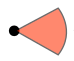
\includegraphics[width=.5\linewidth]{figures/ch04_cws.png}\\ 
Grasp Wrench Space (GWS): alle möglichen Summen aus jeweils einem Wrenchvektor jedes einzelnen Kegels & 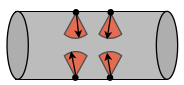
\includegraphics[width=.5\linewidth]{figures/ch04_gws.png}\\
Task Wrench Space (TWS): aufgabenabhängig, hier: Knopf drücken & 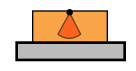
\includegraphics[width=.5\linewidth]{figures/ch04_tws.png}
\end{tabular}
\item Eigenschaften eines Griffs: Widerstand gegen Stöße (beliebiger externer Wrench $w$):
\begin{itemize}
\item Force-closure: $-w$ liegt im GWS
\item Form-closure: geometrische Einschränkung
\end{itemize}
\item Qualitätsmaße für Griffe (Grasp quality measure)
\begin{itemize}
\item Beispiel: größte Hyperkugel um 0, die im GWS liegt
\end{itemize}
\end{itemize}
Griffe werden bei der \textbf{Vorwärtsgriffplanung} in folgenden Schritten berechnet:
\begin{itemize}
\item[1.] Setze Gelenkwinkel des Handmodells vor dem Zugreifen, z.B. prismatischer Kraftgriff
\item[2.] Setze 3d-Handmodell relativ zu Objekt vor dem Anrücken
\item[3.] Bewege Hand auf das Objekt zu
\item[4.] Schließe jeden einzelnen Finger bis auf Kontakt: Einfacher Algorithmus\footnote{Spezialisierte Algorithmen basierend auf Distanz: C2A [Tang2009]}
\begin{itemize}
\item[1.] Schrittweise Änderung der Gelenkwinkel bis Hand komplett geschlossen
\item[2.] Überprüfung der Kollisionen in jedem Schritt → geom. Objektmodell
\item[3.] Bei Kollision: gebe vorherige Gelenkwinkel zurück
\end{itemize}
\item[5.] Bestimme Kraftkegel in allen Kontaktpunkten
\item[6.] Berechne Griffqualität
\item[7.] $\ast$ Iteriere bis Griff mit hoher Griffqualität gefunden
\end{itemize}
\subsubsection*{Vorwärtsplaner: GraspIt! Simulator für Greifbewegungen}
Die Greifbewegung erfolgt nach einem einfachen Algorithmus: Finger schließen bis Kontakt (vgl. \autoref{fig:graspit})
\begin{enumerate}
\item Schrittweise Änderung der Gelenkwinkel bis Hand komplett geschlossen
\item Überprüfung der Kollisionen in jedem Schritt $\rightarrow$ geom. Objektmodell
\item Bei Kollision: gebe vorherige Gelenkwinkel zurück
\end{enumerate}
\begin{figure}[h!]
	\centering
	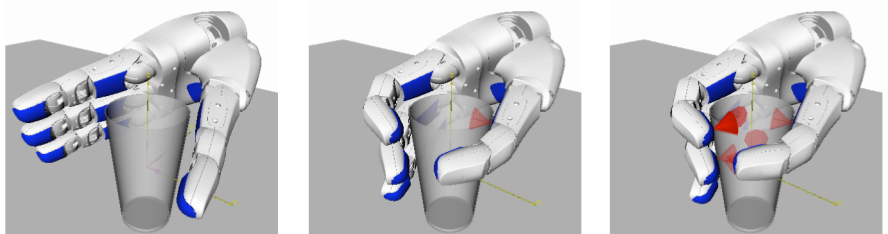
\includegraphics[width=.7\textwidth]{figures/ch04_graspit.png}
	\caption{GraspIt!}
	\label{fig:graspit}
\end{figure}
\begin{itemize}
\item Beliebige Robotersysteme
\item Beliebige Objekte, Hindernisse
\item Verschiedene Qualitätsmaße für Griffe
\item Soft finger contacts
\item Physikengine
\end{itemize}
Ein vorwärtsgerichtetes Greifplanungsverfahren für die Barretthand\footnote{[Miller03]: Automatic Grasp Planning Using Shape Primitives} auf Basis des GraspIt! Simulators läuft folgendermaßen ab:
\begin{itemize}
\item Vorgabe einer Griffform (\Gu preshape \Go, hier zwei vordefinierte preshapes: zylindrisch und kugelförmig)
\item Vorgabe einer Startpose und Anrückbewegung
\item Durchführung des Griffs
\item Evaluation mit Qualitätsmaß
\end{itemize}
Die Bestimmung der Greifstrategie (Preshape und Startlage) erfolgt auf Basis einer Zerlegung des zu greifenden Objekts in Objektprimitive (Kugeln, Zylinder, Kegel, Quader). Dabei existiert eine Vorgabe einer Menge von Greifstrategien für jedes der Objektprimitive. Die Anrückbewegung erfolgt dann linear in $z$-Richtung bis zu einem Kontakt, danach Backtracking. Abbildung \ref{fig:ch04_griffe} zeigt auf der linken Spalte generierte Greifstrategien für verschiedene Objekte und auf der rechten Seite deren Umsetzung.
\begin{figure}[ht]\centering 
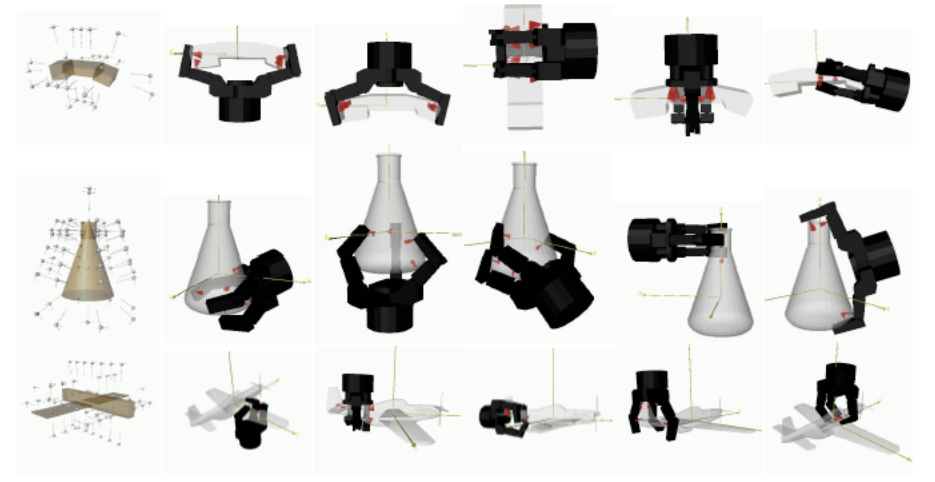
\includegraphics[width=0.5\linewidth]{figures/ch04_griffe.png}
\caption{Greifplanungsverfahren für die Barretthand}
\label{fig:ch04_griffe}
\end{figure}
\newpage
Das \textbf{Lernen von Griffen durch PdV} ist im folgenden noch einmal zusammengefasst:
\begin{itemize}
\item[1.] \underline{Beobachtung des Menschen}
\begin{itemize}
\item Mensch demonstriert Griffbewegung
\item Bestimmung der Griffform basierend auf Cutkosky-Hierarchie, z.B. sphärischer Präzisionsgriff
\item Bestimmung der Anrückbewegung auf das Objekt
\end{itemize} 
\item[2.] \underline{(Vorwärtsgerichtete) Griffplanung zur Bestimmung von Kontaktstellen auf dem Objekt}
\begin{itemize}
\item Abbildung der menschlichen auf eine Roboter-Griffform
\item Abbildung der menschlichen auf eine Roboteranrückbewegung
\item Anrücken an Objekt und Schließen der Hand
\item Bestimmung der Kontaktstellen mit geometrischem Objektmodell
\item Berechnung des gewählten Qualitätsmaßes für Griffe
\end{itemize}
\item[3.] \underline{Ausführung auf dem Robotersystem: Griffkraft manuell nachjustiert}
\end{itemize}